\section{Generative Adversarial Networks}
\subsection{Introduction}
So far, we have seen two generative models, autoregressive models and variational autoencoders. Both of these approaches try to model $\P(x)$; autoregressive models directly maximize the likelihood of the data:
\begin{equation*}
    p_\theta(x) = \prod_{i=1}^N p_\theta(x_i|x_1, \dots, x_{i-1})
\end{equation*}
while variational autoencoders maximize the evidence lower bound:
\begin{equation*}
    \log p_\theta(x) \geq \E_{z\sim q_\varphi(z|x)}\left[\log p_\theta(x|z)\right] - \KL\left(q_\varphi(z|x)\;\middle\|\; p(z)\right)
\end{equation*}
Both of these models have their limitations; autoregressive models are slow to sample from, and variational autoencoders can have blurry samples. Generative adversarial networks (GANs) are a third approach to generative modeling that can generate high-quality samples quickly, by focusing on the problem of generating samples from a distribution instead of trying to explicitly model the distribution.

\subsection{Generator and Discriminator}
Assume that we have acces to some data samples $x_i$ drawn from a certain distribution $p_{\text{data}}$. Our goal is to draw new samples from $p_{\text{data}}$, without trying to access its values. Similarly to variational autoencoders, we assume that each sample is associated to a latent variable $z$ with a simple prior distribution $p(z)$. The idea is to learn a \emph{Generator Network} $G(z)$ that takes a latent variable $z$ as input and outputs a sample $x = G(z)$. $G$ implicitely defines a probability distribution $p_G$ over the samples $x$; we want to learn $G$ such that $p_G$ is as close as possible to $p_{\text{data}}$.

In parallel, we will train a \emph{Discriminator Network} $D$ to perform a classification task: given a sample $x$, $D(x)$ should output the probability that $x$ is a sample from $p_{\text{data}}$ rather than $p_G$. The training of $D$ is supervised: it is trained on both real samples $x_i$ and fake samples $G(z)$, of which we know the labels $0$ and $1$ respectively.
\begin{figure}[H]
    \centering
    \includegraphics[width=.9\textwidth]{gans/generator-discriminator.png}
\end{figure}
We train the Generator $G$ and the Discriminator $D$ in an \emph{adversarial} manner: $G$ tries to fool $D$ by generating samples that are indistinguishable from real samples, while $D$ tries to distinguish between real and fake samples.

\subsection{Training objective}
We will jointly train the Generator $G$ and the Discriminator $D$ with a \emph{minimax game}. A first objective to optimize for is the following:
\begin{equation}
    \min_G\max_D \left(
        \E_{x\sim p_{\text{data}}}\left[\log D(x)\right] + \E_{z\sim p(z)}\left[\log\left(1-D\left(G(z)\right)\right)\right]
    \right)
\end{equation}
The Discriminator wants $D(x)=1$ for real data and $D(x)=0$ for fake data. Therefore, the first inner quantity $\E_{x\sim p_{\text{data}}}\left[\log D(x)\right]$ is the $\log$-likelihood of a real sample being classified as real, while the second inner quantity $\E_{z\sim p(z)}\left[\log\left(1-D\left(G(z)\right)\right)\right]$ is the $\log$-likelihood of a fake sample being classified as fake. The objective of the Discriminator is to maximize both these quantities, while the Generator tries to minimize them.

Let $V(G, D) = \E_{x\sim p_{\text{data}}}\left[\log D(x)\right] + \E_{z\sim p(z)}\left[\log\left(1-D\left(G(z)\right)\right)\right]$. The training loop will consist in alternating between the optimization of $D$ and $G$; for $t\in\iset{0}{T}$:
\begin{enumerate}
    \item Update $D$: \begin{equation*}D\longleftarrow D+\alpha_D\frac{\partial V}{\partial D}\end{equation*}
    \item Update $G$: \begin{equation*}G\longleftarrow G-\alpha_G\frac{\partial V}{\partial G}\end{equation*}
\end{enumerate}
Note that we are not minimizing any overall loss; the generator and the discriminator have their own loss, which depend on each other and is usually not monotonically decreasing.

In practice, at the start of training, the generator performs quite poorly while the dicriminator can easily tell apart real and fake data, making $D(G(z))$ very close to $0$. This usually leads to a vanishing gradient for $G$. To avoid this, instead of training $G$ to minimize $\log\left(1-D(G(z))\right)$, we train it to minimize $-\log D(G(z))$.

\subsection{Optimality}
We hope that jointly training $G$ and $D$ will make the generator's distribution $p_G$ converge to $p_{\text{data}}$. We will analytically derive the optimal discriminator and generator to show that this is the case.

First, note that:
\begin{align*}
    &\min_G\max_D \left(
        \E_{x\sim p_{\text{data}}}\left[\log D(x)\right] + \E_{z\sim p(z)}\left[\log\left(1-D\left(G(z)\right)\right)\right]
    \right) \\
    = &\min_G\max_D \left(
        \E_{x\sim p_{\text{data}}}\left[\log D(x)\right] + \E_{x\sim p_G}\left[\log\left(1-D(x)\right)\right]
    \right) && \text{(change of variables)} \\
    = &\min_G\max_D
        \int_X \left( p_{\text{data}}(x)\cdot\log D(x) + p_G(x)\cdot\log\left(1-D(x)\right) \right) \dd x
     && \text{(definition of $\E$)}
\end{align*}

We can now derive the optimal discriminator $D_G^*$. Note that the quantity inside the integral,
\begin{equation*}
    p_{\text{data}}(x)\cdot\log D(x) + p_G(x)\cdot\log\left(1-D(x)\right)
\end{equation*}
is of the form:
\begin{equation*}
    f(y) = a\cdot\log y + b\cdot\log(1-y)
\end{equation*}
We have that $f'(y) = \frac{a}{y} - \frac{b}{1-y} = 0$ when $y = \frac{a}{a+b}$. Therefore, the optimal discriminator is:
\begin{equation*}
    D_G^*(x) = \frac{p_{\text{data}}(x)}{p_{\text{data}}(x) + p_G(x)}
\end{equation*}

We can continue the computation to find the optimal generator $G^*$. We have:
\begin{align*}
    &\min_G\max_D \left(
        \E_{x\sim p_{\text{data}}}\left[\log D(x)\right] + \E_{z\sim p(z)}\left[\log\left(1-D\left(G(z)\right)\right)\right]
    \right) \\
    = &\min_G
        \int_X \left( p_{\text{data}}(x)\cdot\log D^*_G(x) + p_G(x)\cdot\log\left(1-D^*_G(x)\right) \right) \dd x \\
    = &\min_G
        \int_X \left( p_{\text{data}}(x)\cdot\log\left(\frac{p_{\text{data}}(x)}{p_{\text{data}}(x) + p_G(x)}\right) + p_G(x)\cdot\log\left(1-\frac{p_{\text{data}}(x)}{p_{\text{data}}(x) + p_G(x)}\right) \right) \dd x \\
    = &\min_G
        \left( \E_{x\sim p_{\text{data}}}\left[\log\frac{p_{\text{data}}(x)}{p_{\text{data}}(x) + p_G(x)}\right] + \E_{x\sim p_G}\left[\log \frac{p_{\text{data}}(x)}{p_{\text{data}}(x) + p_G(x)}\right] \right) \\
\end{align*}
To obtain a simpler expression, we multiply by a factor $2$ to make the Kullback-Leibler divergence appear:
\begin{align*}
    &\phantom{=}\min_G\max_D \left(
        \E_{x\sim p_{\text{data}}}\left[\log D(x)\right] + \E_{z\sim p(z)}\left[\log\left(1-D\left(G(z)\right)\right)\right]
    \right) \\
    &=\min_G
        \left( \E_{x\sim p_{\text{data}}}\left[\log\frac{2\cdot p_{\text{data}}(x)}{p_{\text{data}}(x) + p_G(x)}\right] + \E_{x\sim p_G}\left[\log \frac{2\cdot p_{\text{data}}(x)}{p_{\text{data}}(x) + p_G(x)}\right]\right) - \log4 \\
    &= \min_G
        \left(\KL\left(
            p_{\text{data}}\;\middle\|\;\frac{p_{\text{data}}+p_G}{2}
        \right) + \KL\left(
            p_G\;\middle\|\;\frac{p_{\text{data}}+p_G}{2}
        \right)\right) - \log4 \\
    &= 2\times\min_G \JSD\left(p_{\text{data}}\;\middle\|\; p_G\right) - \log4 \\
\end{align*}
where $\JSD$ is the Jensen-Shannon divergence\footnote{
    The Jensen-Shannon divergence is defined as $\JSD\left(p\;\middle\|\; q\right) = \frac{1}{2}\KL\left(p\;\middle\|\;\frac{p+q}{2}\right) + \frac{1}{2}\KL\left(q\;\middle\|\;\frac{p+q}{2}\right)$.
}.
Hence, since the Jensen-Shannon divergence is always non-negative, and zero if and only if the two distributions are equal, $p_{\text{data}} = p_G$. Therefore, the optimal generator for the optimal $D$ is the data distribution itself.

Even though we have no guarantee that we can actually represent the optimal $D$ and $G$, this shows that the GAN training objective is well-posed and can converge to the optimal solution if the networks are expressive enough.

\subsection{DC-GAN}
A direct extension to the basic generative adversarial architecture is the Deep Convolutional GAN (DC-GAN). The generator and discriminator are both convolutional neural networks, which allows them to learn spatial hierarchies of features.
\begin{figure}[H]
    \centering
    \includegraphics[width=.8\textwidth]{gans/dcgan.png}
    \caption{DC-GAN architecture.}
\end{figure}

\subsection{Results}
\subsubsection{Image generation}
Generated samples from DC-GANs can be of very high quality. For example, the following images were generated by a DC-GAN trained on the LSUN bedrooms dataset:
\begin{figure}[H]
    \centering
    \includegraphics[width=.9\textwidth]{gans/dcgan-bedrooms.png}
    \caption{Samples generated by a DC-GAN trained on the LSUN bedrooms dataset.}
\end{figure}
Those images capture the complexity of the dataset, with realistic textures and shapes.

\subsubsection{Image interpolation}
Similarly to variational autoencoders, GANs generate images from a given latent vector. This allows for smooth interpolation between two generated images. For example, the following images were generated by interpolating between two latent vectors:
\begin{figure}[H]
    \centering
    \includegraphics[width=.9\textwidth]{gans/dcgan-interpolation.png}
    \caption{Interpolation between two images generated by a DC-GAN.}
\end{figure}

\subsubsection{Conditional GANs}
We previously made the distinction between unconditional and conditional generative models. While unconditional generative models learn the distribution $\P(x)$, conditional generative models learn the distribution conditioned on the data label, that is $\P(x|y)$.

To build a conditional GAN, we simply add the label $y$ as input to both the generator and the discriminator. The generator will generate samples $x = G(z, y)$, while the discriminator will classify samples $x$ as real or fake given the label $y$.

A commonly used method to input label information to the generator is to use \emph{conditional batch normalization}. The idea is to learn a separate scale and shift ($\gamma$ and $\beta$) for every label, which are applied to the batch normalization layer. This allows the generator to learn different statistics for each label.

Recall that a standard normalization layer computes the following quantities:
\begin{equation*}
    \mu_j = \frac{1}{N}\sum_{i=1}^N x_{i, j} \qquad
    \sigma_j^2 = \frac{1}{N}\sum_{i=1}^N (x_{i,j}-\mu_j)^2 \qquad
    \hat{x}_{i,j} = \frac{x_{i,j}-\mu_j}{\sqrt{\sigma^2_j+\epsilon}} \qquad
    y_{i,j} = \gamma_j\hat{x}_{i,j}+\beta_j
\end{equation*}
where $\gamma$ and $\beta$, the scale and shift vectors, are parameters learned during training and used as constants during inference. In conditional batch normalization, we learn a separate $\gamma^y$ and $\beta^y$ for each label $y$, resulting in the following equations:
\begin{equation*}
    \mu_j = \frac{1}{N}\sum_{i=1}^N x_{i, j} \qquad
    \sigma_j^2 = \frac{1}{N}\sum_{i=1}^N (x_{i,j}-\mu_j)^2 \qquad
    \hat{x}_{i,j} = \frac{x_{i,j}-\mu_j}{\sqrt{\sigma^2_j+\epsilon}} \qquad
    y_{i,j} = \textcolor{red}{\gamma_j^y}\hat{x}_{i,j}+\textcolor{red}{\beta_j^y}
\end{equation*}

This allows to train GANs on datasets with multiple classes, and generate samples conditioned on a given label. For example, the following images were generated by a conditional GAN trained on the ImageNet dataset:
\begin{figure}[H]
    \centering
    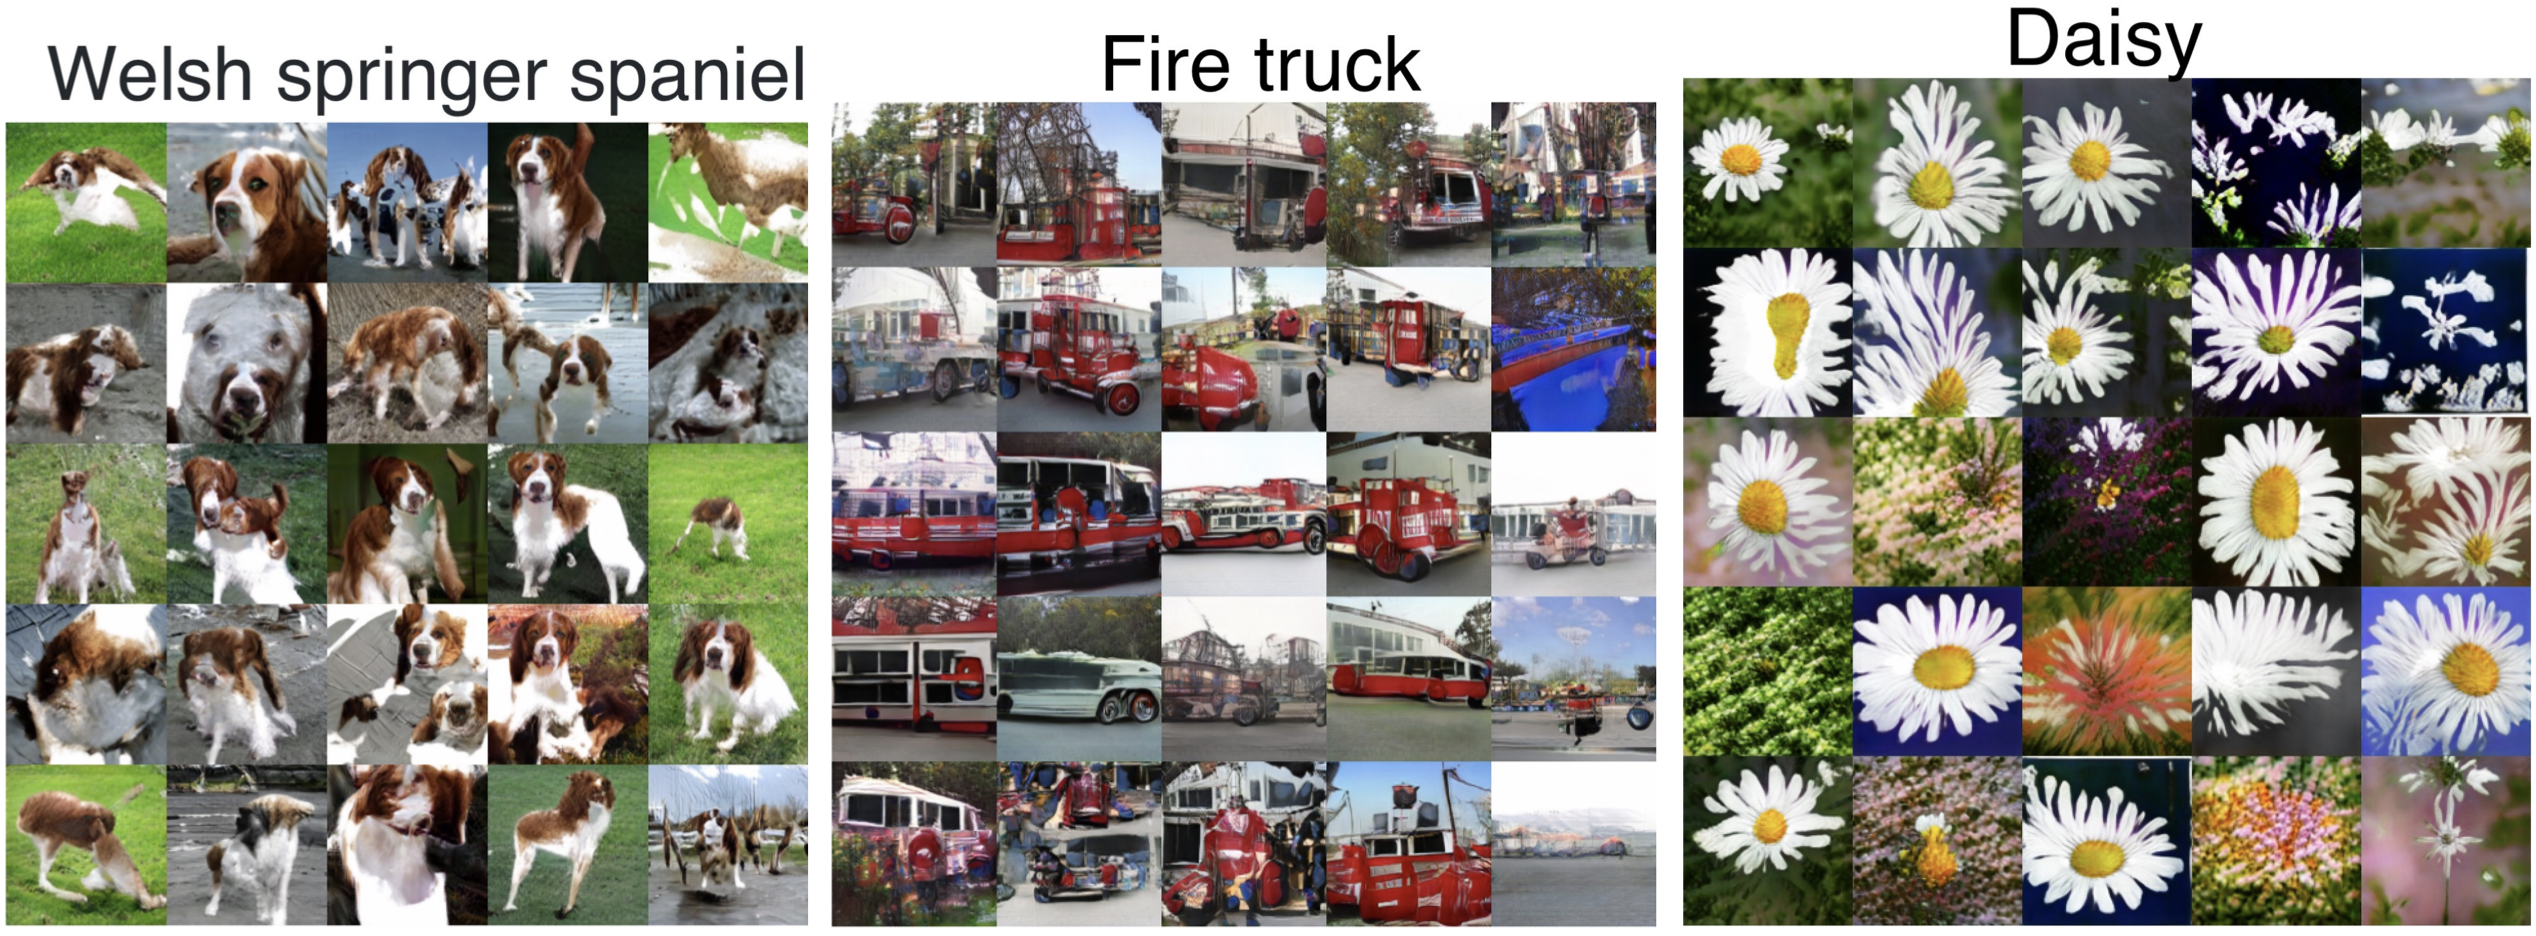
\includegraphics[width=.9\textwidth]{gans/conditional-gan.png}
\end{figure}

\subsection*{Generative Adversarial Networks: Summary}
Generative Adversarial Networks is an approach in which we jointly train two networks to generate samples from a distribution. The Generator $G$ generates samples from a latent variable $z$, while the Discriminator $D$ tries to distinguish between real and fake samples. $G$ attempts to fool $D$, while $D$ tries to classify the data correctly.

GANs have many applications, from the generation of high-quality images to the generation of music or text. They can be extended to conditional GANs, which generate samples conditioned on a given label.

\newpage